\chapter{Background Research}
\label{chapter2}

\section{Robot Operating System (ROS)}

The Robot Operating System or ROS, is a flexible framework for writing robot software. It offers libraries aiming at simplifying common robotics tasks \cite{website:aboutROS}, which otherwise would be too complex and daunting to achieve in such a broad field.

ROS is a collaborative and open-source project empowering the expertise of some of the best robotics institutions, laboratories and individuals around the globe \cite{website:aboutROS}, making ROS a well rounded framework for all types of robotics challenges. 

ROS comes in many versions. This project will make extensive use of the ROS Indigo Igloo version which targets the Ubuntu 14.04 (LTS) release.

\section{Gazebo}

Gazebo is a 3D simulator engine able to render accurately and efficiently complex indoor and outdoor environments \cite{website:Gazebo}, thereby speeding up the development process by being able to test robotics algorithms and modules via its wide and rich library of robot models and environment \cite{website:Gazebo}, without the need of particular robotics hardware.

For this project Gazebo's TIAGo extension by PAL ROBOTICS was used.

\begin{figure}[!htbp]
\begin{center}
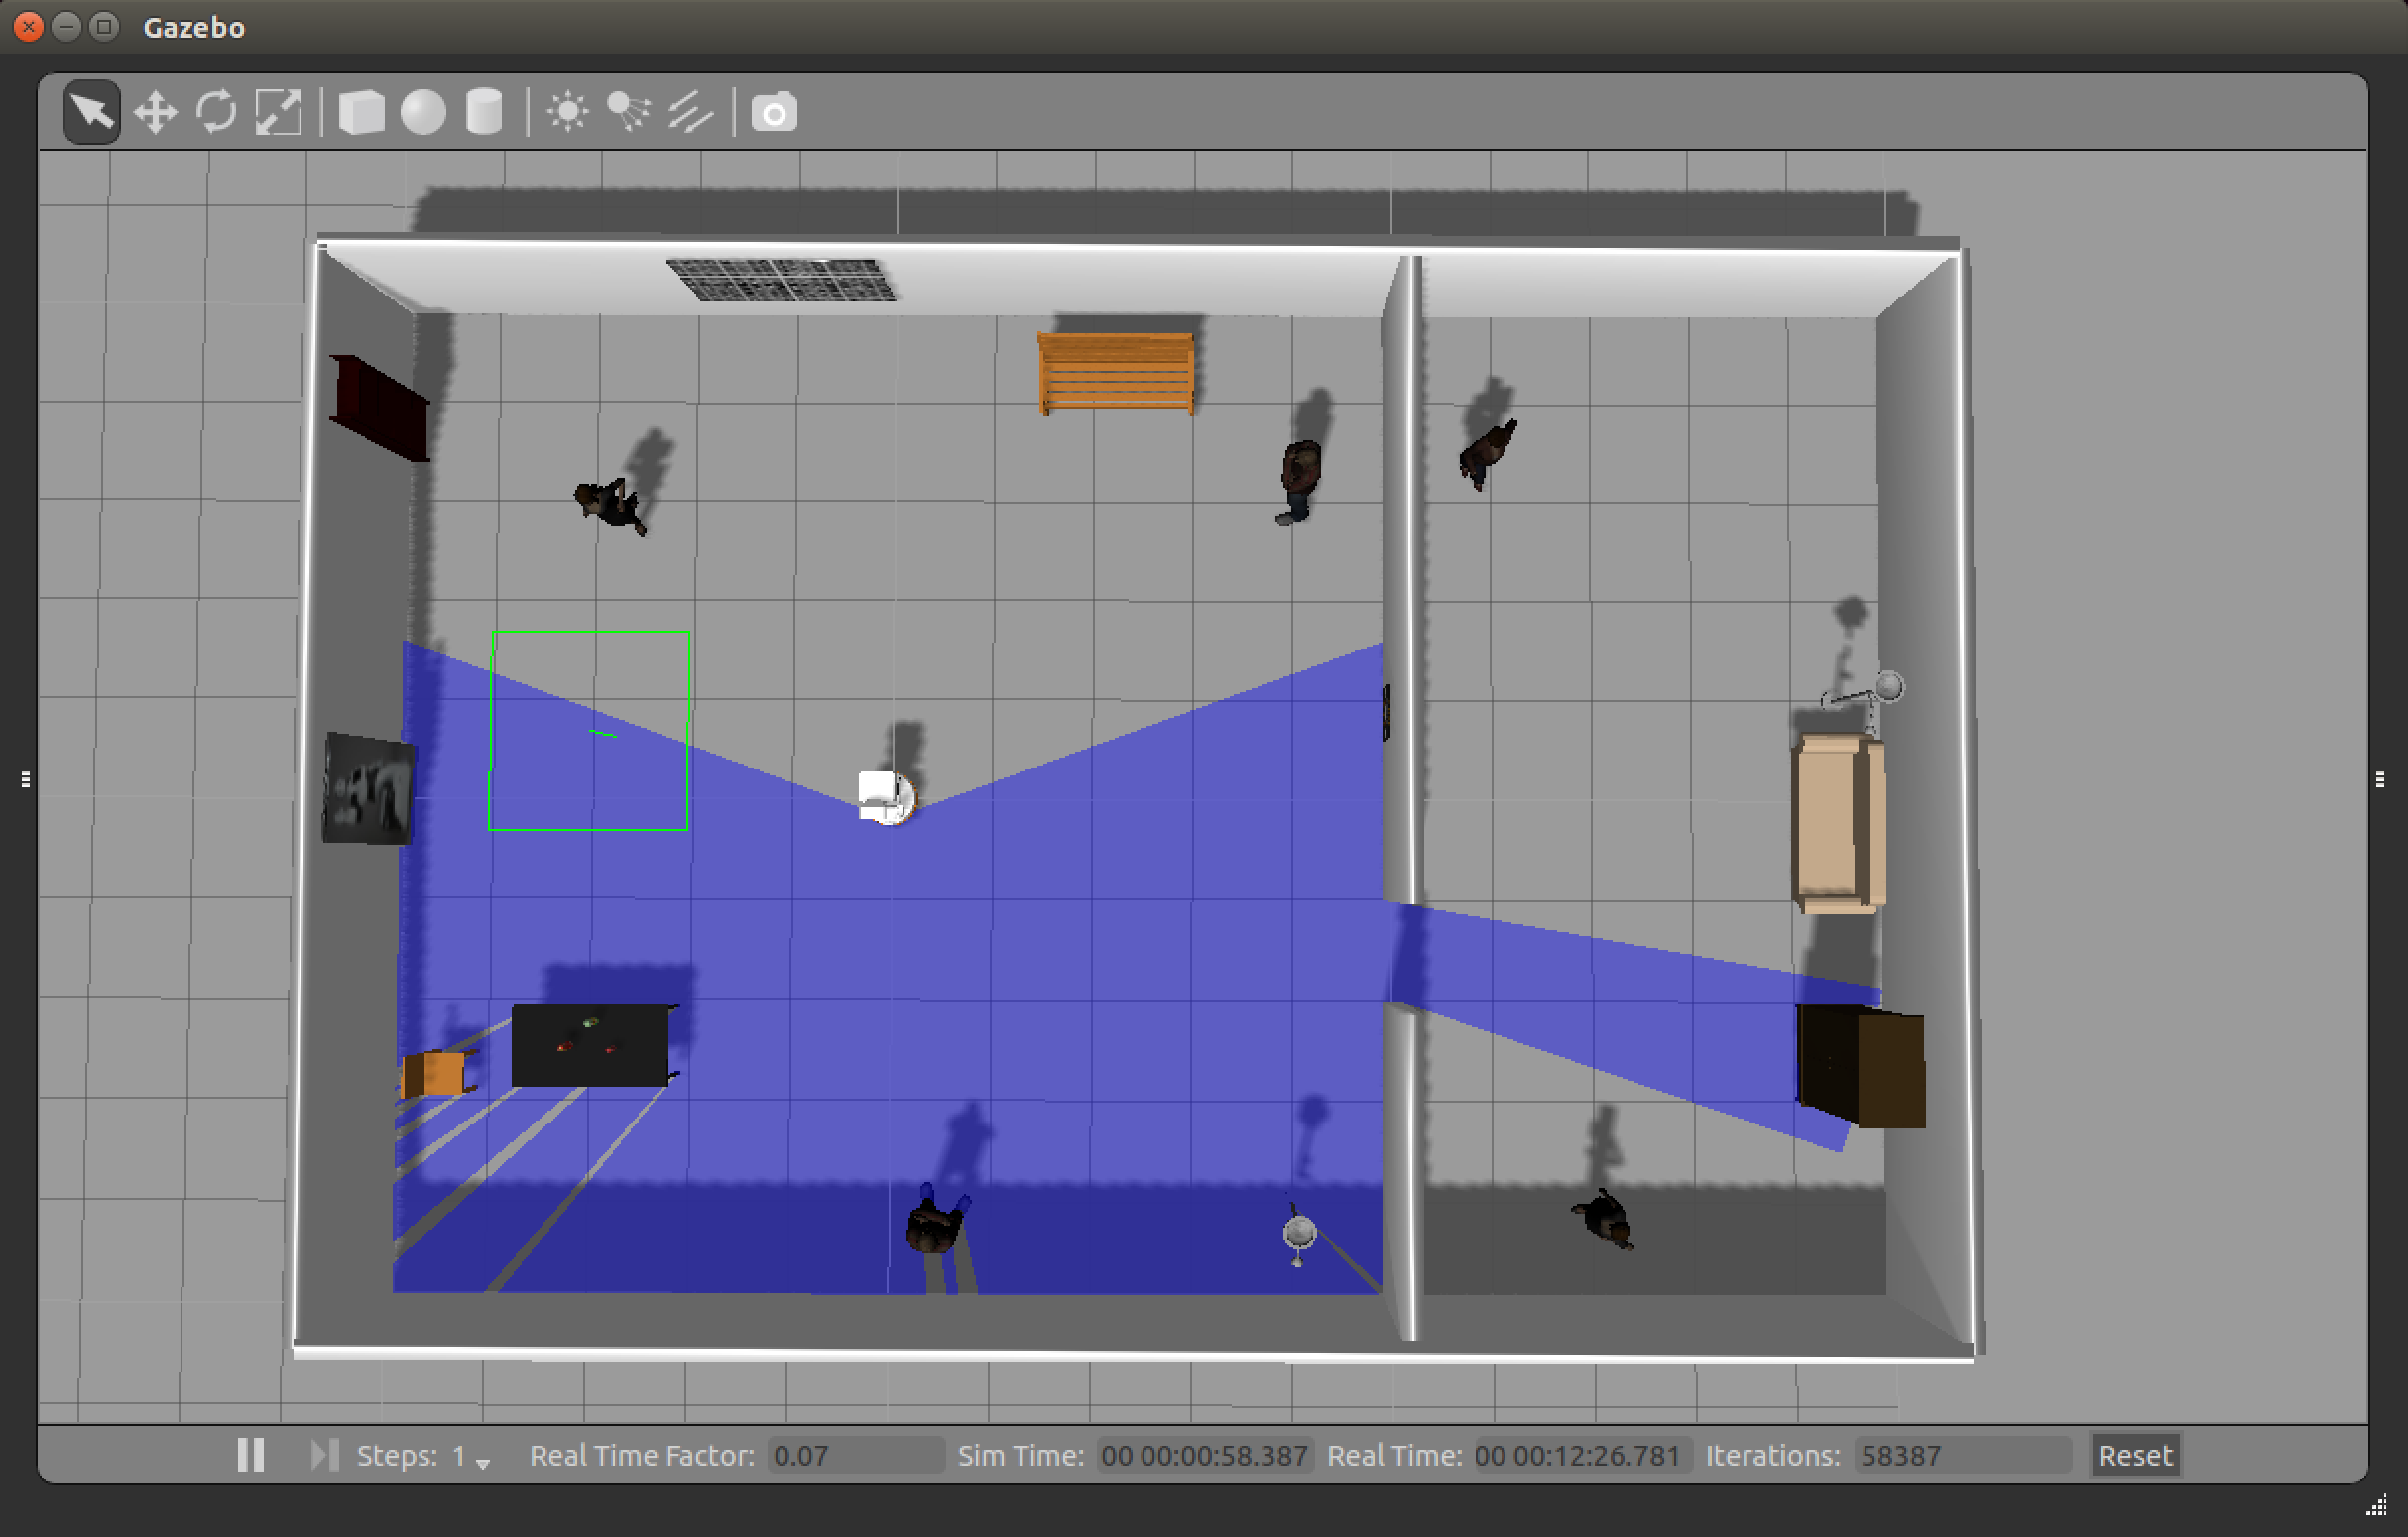
\includegraphics[width=\linewidth]{images/chapter2_gazebo_screenshot1.png}
\end{center}
\caption{Gazebo Simulator (Office Environment)}
\label{fig:gazebo_screenshot1}
\end{figure}

\begin{figure}[!htbp]
\begin{center}
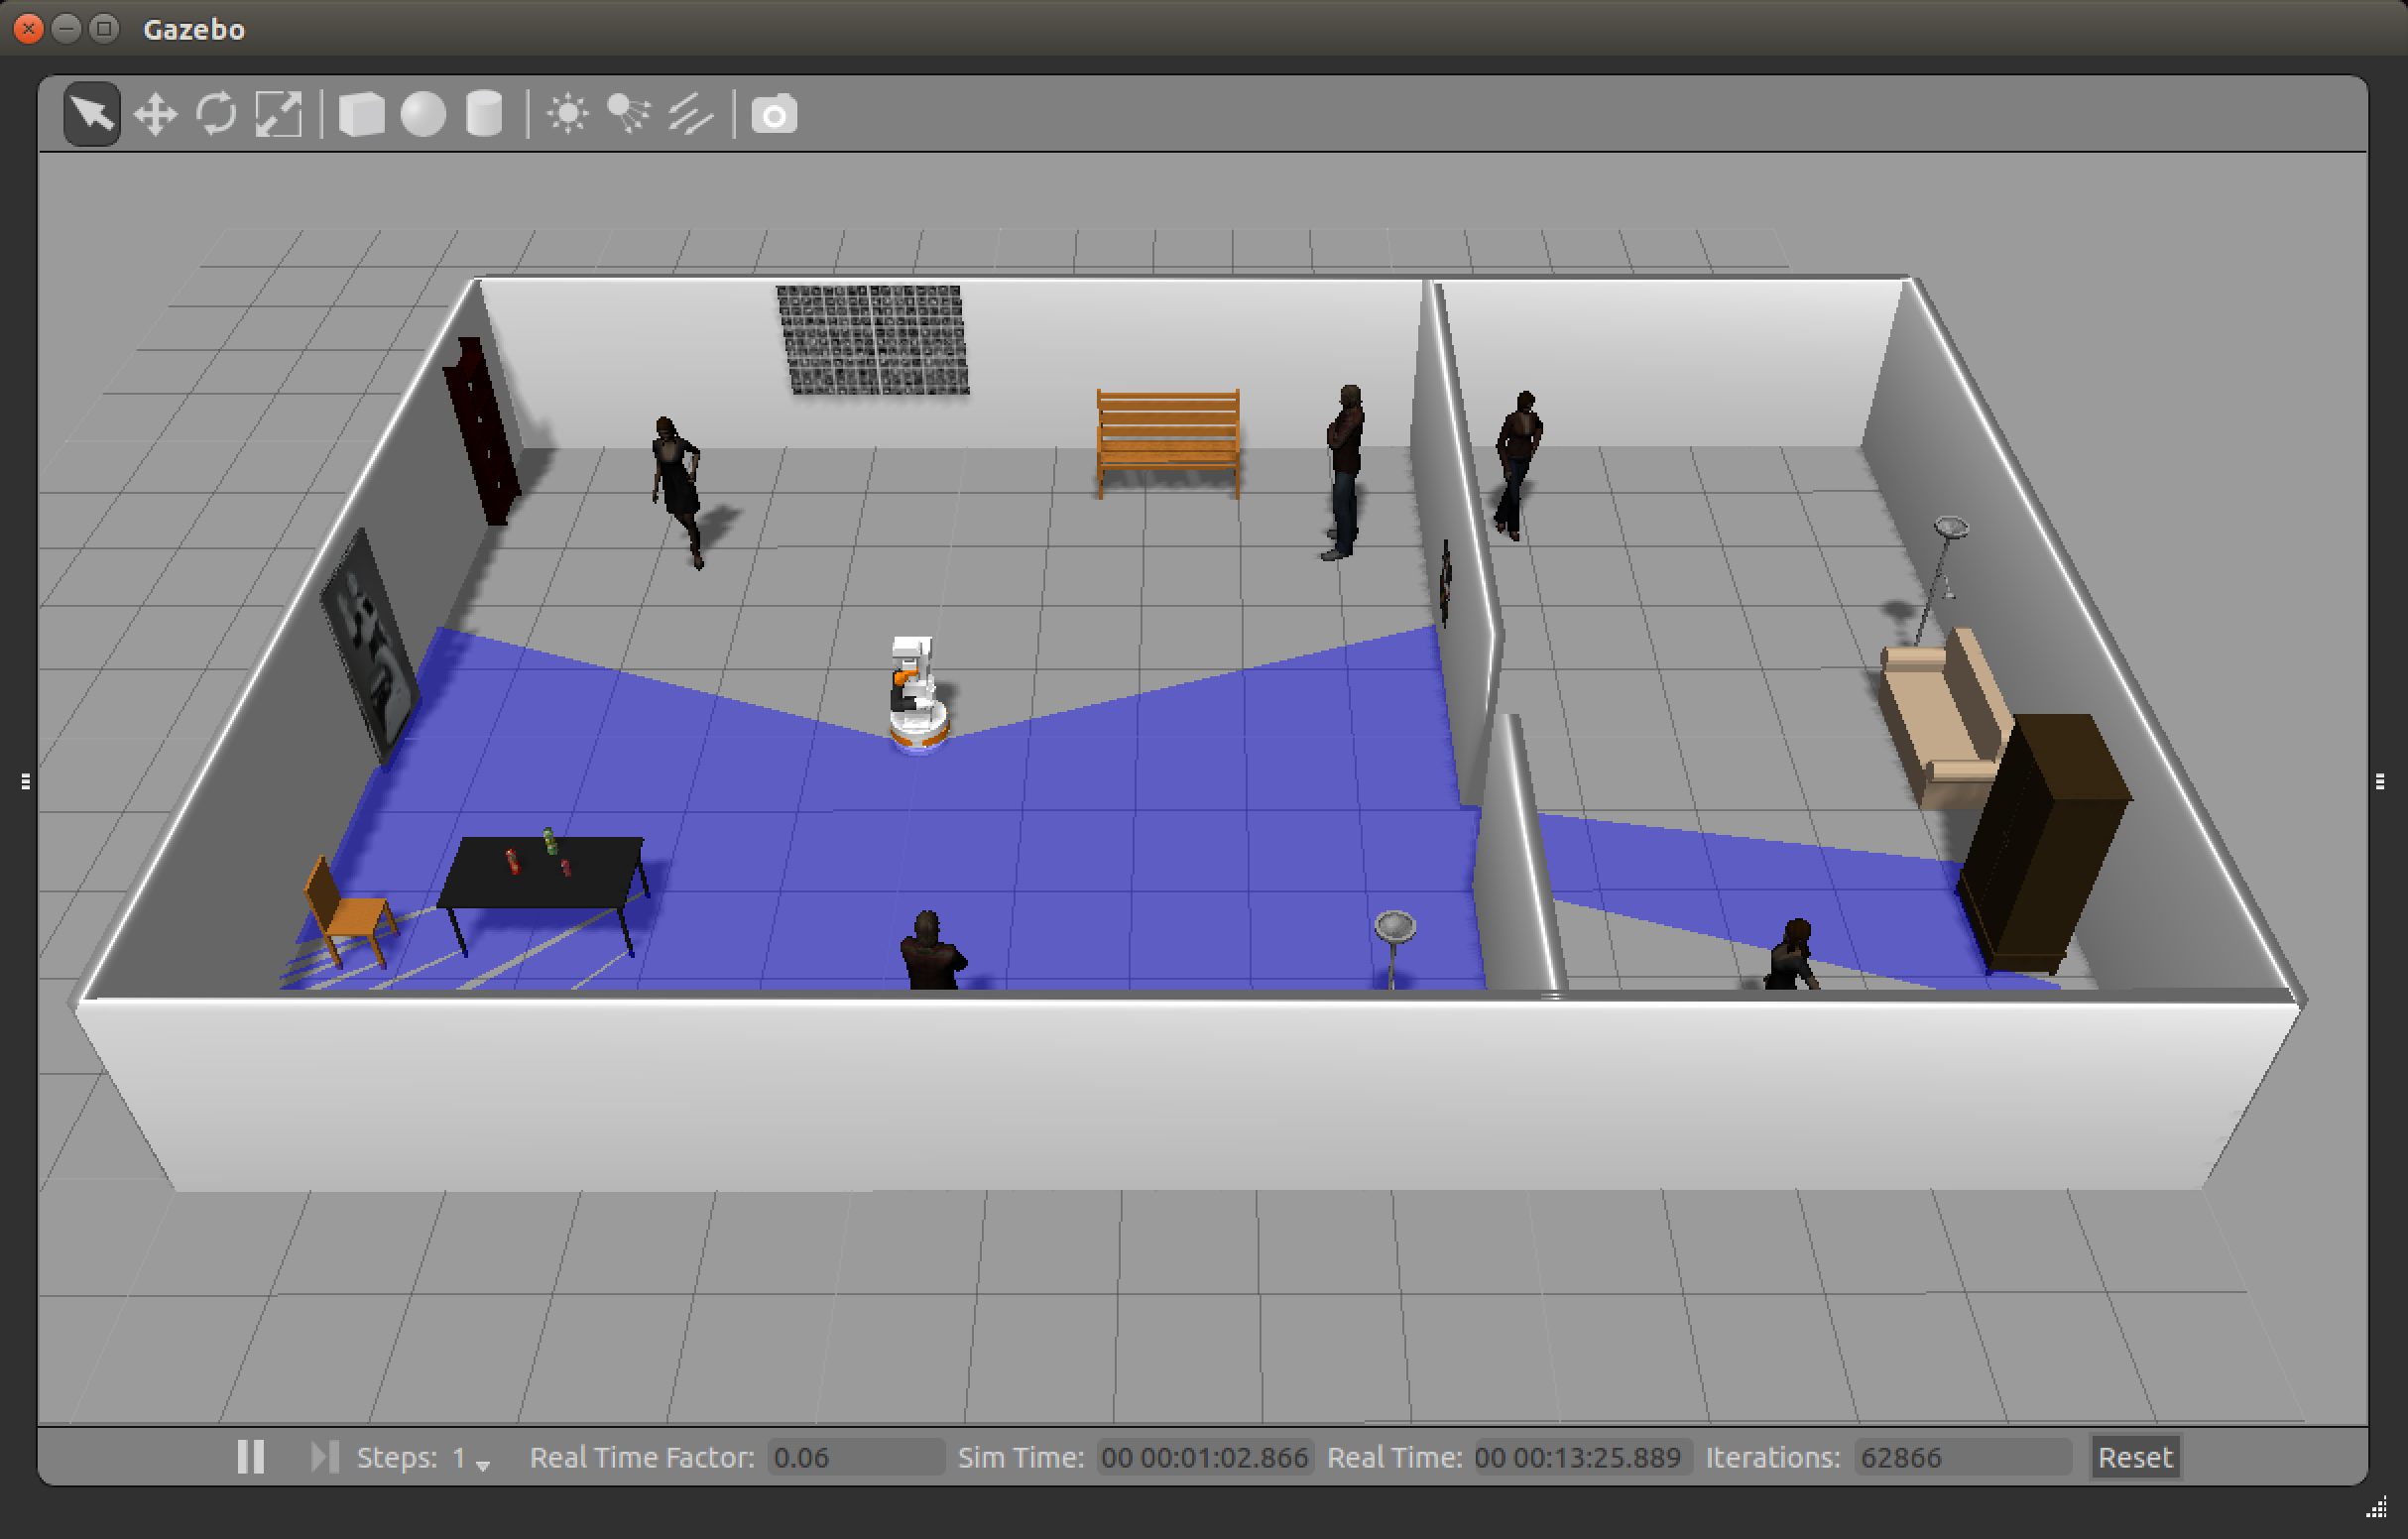
\includegraphics[width=\linewidth]{images/chapter2_gazebo_screenshot2.png}
\end{center}
\caption{Gazebo Simulator (Office Environment)}
\label{fig:gazebo_screenshot2}
\end{figure}

\section{RVIZ}

RVIZ is a 3D visualisation tool that provides information about what the robot is seeing, thinking and doing. Developing robotics application is by itself a daunting task, but without exactly knowing what the robot thinks is going on in the real world it rises the level of complexity, as trying to debug only via numerical data is rather complicated especially at higher number of dimensions which is common in the robotics field \cite{website:RVIZ}. 

Other important features that RVIZ offers via its modules are point cloud visualisation, laser-scan readings, coordinate frames as well as topological maps, obstacles data and current path visualisation when using the ROS navigation stack making of RVIZ a powerful tool for this project and generally for the development of robot capabilities and research \cite{website:RVIZ}.

\begin{figure}[!htbp]
\begin{center}
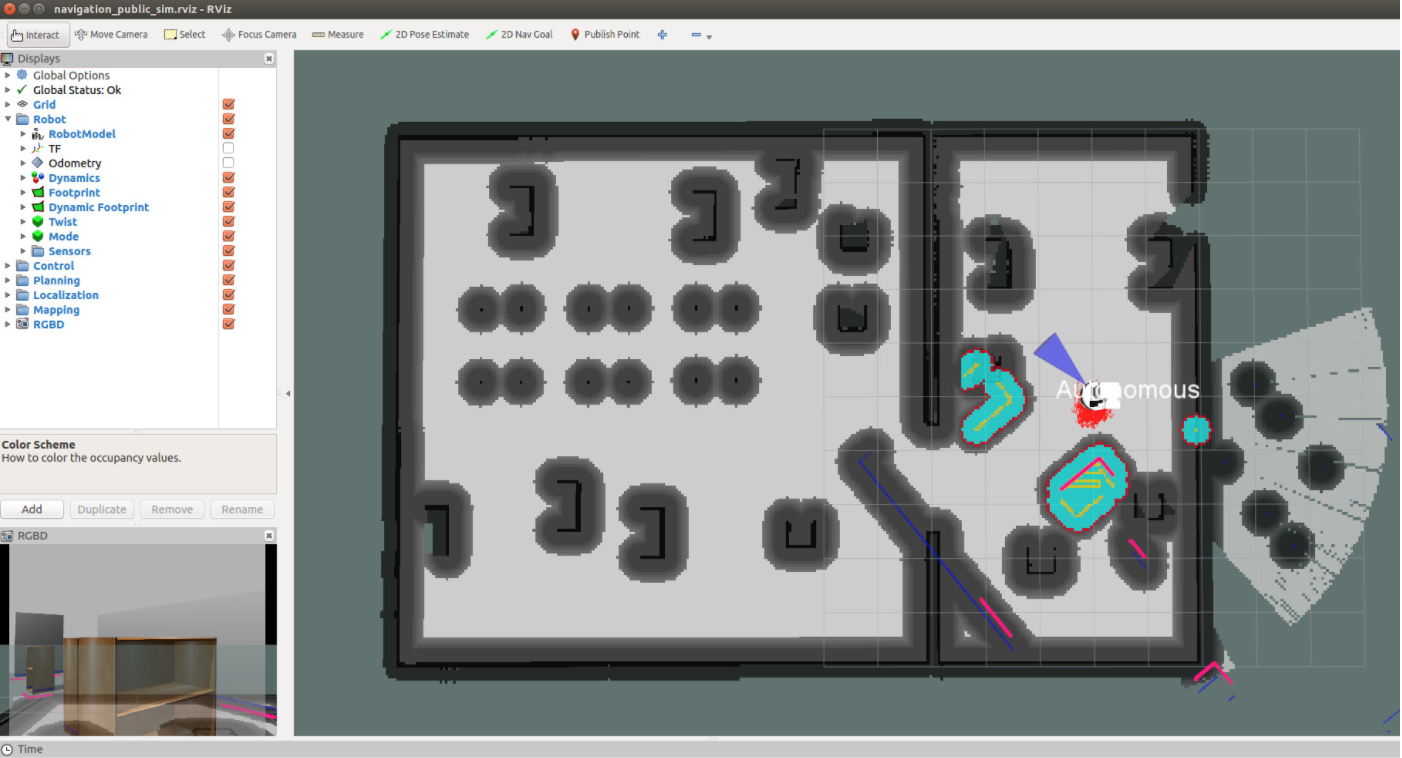
\includegraphics[width=\linewidth]{images/RVIZ_screenshot.png}
\end{center}
\caption{RVIZ in action.}
\label{fig:rviz_screenshot}
\end{figure}

\section{TIAGO}

TIAGO, a robot by PAL Robotics, is a the main and only robot used throughout the project given its characteristics and sensory devices treated in the coming sections. 

TIAGO is a service robot, designed to work in indoor environments \cite{website:TIAGo}, hence fitting our project aim of creating a ROS package for a robust human pose estimation which can be used to maneuver and interact around and with humans, although not limited to it only.

Moreover, TIAGO's size and technical features make it an ideal platform for the project, combining many of the necessary aspects for the positive outcome of the task, including RGB-D camera for 2D person detection and depth estimation, Laser range finder for person's leg detection and a Differential-drive base to move around the environment.

\begin{figure}[!htbp]
\begin{center}
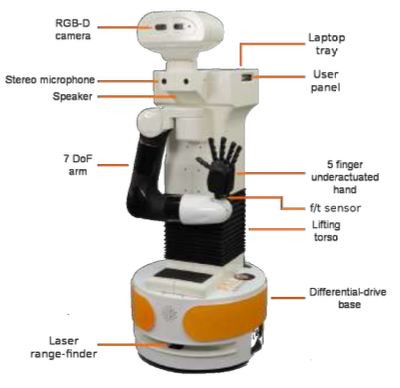
\includegraphics[width=3cm,height=4cm,keepaspectratio]{images/tiago_components.png}
\end{center}
\caption{TIAGO and its components (Image from PAL ROBOTICS \cite{website:TIAGOWEBSITE}).}
\end{figure}

\subsection{RGB-D}

The RGB-D sensor found on TIAGO, like other similar sensors such as the Kinect, provides both colour information as well as the estimated depth for each pixel in the two dimensional colour image.

To achieve this, TIAGO uses an RGB camera and a special camera sensor. In fact, the sensor firsts projects an infrared speckle patters which is ultimately captured by an infrared sensor component in it, and compared part-by-part to reference patterns stored in the device. The capture patterns are of known depth \cite{paper:RGB-D}.

A further step is still needed to obtain the corresponding depth in the RGB image, which is to correlate the data provided by the infrared sensor to a calibrated RGB camera, known as the Point Cloud, a three dimensional space collection of points \cite{paper:RGB-D}.

TIAGO already comes with an RGB-D camera integrated. An Astra model with a minimum and maximum sensor range of 0.6m and 8m.

\subsection{Lasers}

Laser-range finders is another important sensory device for this project. This technology is based on beam reflection and the time of flight.

The laser sends a pulse of light to target and measures the time it takes for the reflection to come back, i.e. the reflection \cite{website:lasers}. Therefore, by knowing the speed at which the beam travels (speed of light) and the time takes for the pulse of light to be emitted and come back, the distance is easily computable using the velocity equation.

TIAGO comes with an integrated laser-range finder with a range of 0.05-25 m and a 180 degree field of view. The frequency of the signal is of 15Hz.

\section{Human Detection}

Given the final objective of creating a ROS package able to estimate humans' position in the environment, a human detection module able to perform such detections on the available RGB sensory data is critical to the good development of the project.

Human detection is a popular and challenging task, given the wide range of features to be considered: skin colour and adopted human pose among others. Therefore, two possible ways of achieving the task have been identified. The first one uses a combination of image gradients and Support Vector Machine (SVM) machine learning model to classify whether humans are present in the image. The second approach is based on deep neural networks, and their ability to carry on object detection with high accuracy.

The two approaches will be considered in this chapter only from a theoretical and algorithmic point of view, thereby highlighting the mechanics of both models and the claimed accuracy and performance results from the respective papers. A more thorough experimentation will be carried on these during the implementation sprints, and a more in depth review will be given in terms of actual performance in the Implementation chapter.

\subsection{HOG (Histogram of Oriented Gradients)}

The Histogram of Oriented Gradients or HOG uses the below shown chain of feature extraction for the classification task.

\begin{figure}[!htbp]
\begin{center}
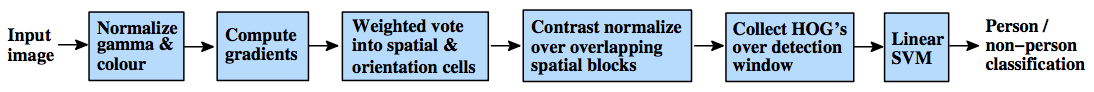
\includegraphics[width=\linewidth]{images/hog_chain.png}
\end{center}
\caption{HOG classification chain (Image taken from: \cite{paper:dalal2005histograms})}
\label{fig:hog_chain}
\end{figure}

The method carries its evaluation on contrast-normalised images to obtain well-contrasted images, as lighting variations and intensities are a key variable for a successful classification. After the input image has been normalised, local histograms of image gradient orientations are extracted by a sliding detection window over the image. The computed vectors are then added to the overall histogram used to identify the presence of humans in the image through a classification task run on SVMs, based on the idea that object appearance and shape can be characterised by the distribution of local intensity gradients and the edge directions \cite{paper:dalal2005histograms}.

The histogram based representation does offer some advantages, mainly it is robust to geometric and photometric transformations. Moreover possible translations or rotations do make little difference if these are smaller than the orientation bin size \cite{paper:dalal2005histograms}.

The descriptor has been tested on the MIT pedestrian database \cite{paper:dalal2005histograms} where it received  perfect detection results and on a custom dataset where instances are standing, but do appear on a variety of orientations and backgrounds however still outperforming other models like Haar Wavelets and PAC-SIFT \cite{paper:dalal2005histograms}.

In conclusion, from the results presented in the paper, the HOG based human detection task should well-perform in the task of detecting humans in RGB data in a reasonable computational time as the image to be searched will be of contained resolution.

\subsection{Deep Learning}

Deep learning is a subset of Machine Learning which has became a common approach to solve computer vision problems, since AlexNet in 2012 managed to improve object-detection accuracy using deep neural networks thanks to the increased availability of training data and most importantly the boost in performance of GPUs computations.

Yann Lacun, Yoshua Benjo and Geoffrey Hinton defined deep learning as a computational model composed of multiple processing layers able to learn the representation of data with multiple levels of abstraction \cite{paper:lecun2015deep}. Such methods have drastically improved the state-of-the-art in tasks like speech recognition, object recognition and object detection by iteratively discovering large data sets' structure using the backpropagation algorithm which helps the neural network update its parametric parameters \cite{paper:lecun2015deep}.

In particular three main models have been identified, able to perform object detection at a high level of accuracy:

\begin{enumerate}
  \item YOLO (You Only Look Once) \cite{paper:YOLO}
  \item Faster R-CNN \cite{paper:FRCNN}
  \item SSD (Single Shot Multibox Detector) \cite{paper:SSD}
\end{enumerate}

However, given the subtle difference in the classification accuracy of the aforementioned neural networks, the SSD model has been chosen out of the three for its computational efficiency and therefore its speed of detection as well as its ease to be embedded in a system. Moreover, the mobileNet version of the model will be used for its optimisation behaviour on power constrained devices.

\subsubsection{SSD Overview}

The SSD model is a single deep neural network able to detect various objects in a scene, by discretizing the output space with bounding boxes over different aspect ratios and scales per feature map (i.e. activation layer) \cite{paper:SSD}. During the feed-forward prediction process scores are generated for the presence of each object category in each bounding box along with an adjustment to the bounding boxes' to better match the object shape \cite{paper:SSD}. The network also combines various feature maps predictions with different resolutions to handle objects of various sizes. Moreover, the network classification process is simpler than other state-of-the-art models such as Faster R-CNN, as the former does not require proposal regions and subsequent pixel resampling stages, thereby encapsulating all required computations in a single network making of the SSD easy to train and straightforward to integrate into systems that require a detection component \cite{paper:SSD}, which is exactly our case.

\subsubsection{SSD Architecture}

Current state-of-the-art object detection systems are variances of the same detection process, which includes the following steps \cite{paper:SSD}:

\begin{enumerate}
  \item Hypothesize bounding boxes
  \item Pixel or features re-sampling
  \item Classification
\end{enumerate}

Although the above pipeline has proved to obtain great accuracy results, it has the major drawback of being too computationally expensive for real-time applications \cite{paper:SSD}. The SSD model improves upon Faster R-CNN \cite{paper:FRCNN} and YOLO \cite{paper:YOLO} by removing the need for bounding box proposals and the resampling process while still retaining the same accuracy performance using separate small convolutional filters applied at different aspect ratio detections \cite{paper:SSD}. These  filters are also applied to multiple feature maps from the later stages of the network in order to perform detection at multiple scales \cite{paper:SSD}.

\begin{figure}[!htbp]
\begin{center}
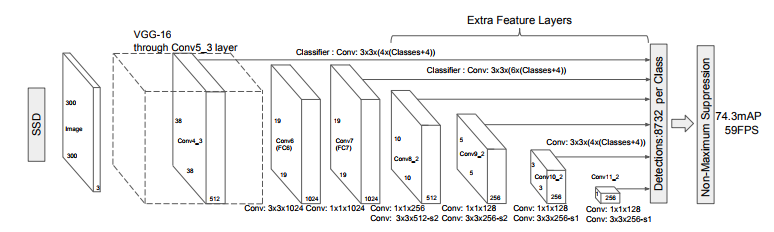
\includegraphics[width=\linewidth]{images/ssd_architecture.png}
\end{center}
\caption{SSD Model (Image taken from: \cite{paper:SSD})}
\label{fig:sshModel}
\end{figure}

The SSD architecture presents a standard base network (VGG-16) used for high quality image classification, upon which auxiliary layers are added to produce detections with the following key features:

\begin{enumerate}
  \item Multi-scale feature maps
  \item Convolutional predictors
  \item Default boxes and aspect ratios
\end{enumerate}

\textbf{Multi-scale feature maps}

Convolutional feature layers are added at the end of the truncated BASE network with the aim of progressively decreasing the input image size, hence allowing for detections at multiple scales \cite{paper:SSD}. Different convolutional models are used for each feature layer \cite{paper:SSD}.

\textbf{Convolutional predictors}

Each added feature layer on top of the base network can produce a fixed set of detection predictions using the previously mentioned convolutional filters \cite{paper:SSD}. Generally speaking a feature layer of size m x n with p channels requires a 3 x 3 x p kernel to produce either a score for a category or a bounding box offset relative to a default box position for each feature map location \cite{paper:SSD}.

\textbf{Default boxes and aspect ratios}

A set of default bounding boxes is associated for each feature map cell, for multiple feature maps at the top of the network (straight after the base network truncation \cite{paper:SSD}. At each feature map cell the offsets relative to the default box shapes as well as the per-class scores indicating the presence of a class instance in each of those boxes \cite{paper:SSD}. Specifically, for each box out of k, the \textit{c} class score is computed as well as the 4 offsets (for each discretized point of the original image 4 bounding boxes are draw with different aspect ratios) \cite{paper:SSD}.

\begin{figure}[!htbp]
\begin{center}
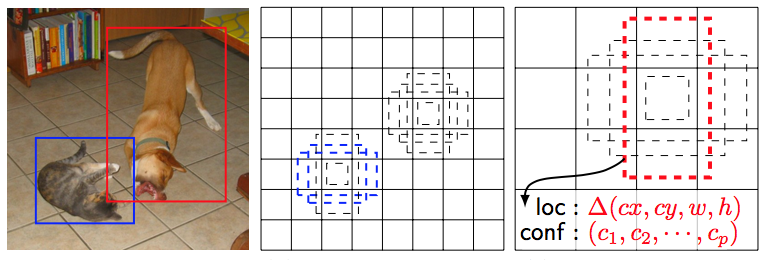
\includegraphics[width=\linewidth]{images/gt_boxes.png}
\end{center}
\caption{Ground truth, feature maps, offset computation(Image taken from: \cite{paper:SSD}).}
\label{fig:ssdGT}
\end{figure}

\subsubsection{MobileNets}

MobileNet provides an efficient network architecture in order to build small and low latency models that can be easily embedded in vision applications running on limited devices \cite{paper:MobileNets}. In fact, although the SSD model is relatively computationally lightweight compared to other state-of-the-art models it is still not enough to carry real-time detections on computationally limited platforms.

The MobileNet structure is built on top of a depthwise separable convolutions except for the first layer which is full convolutional layer \cite{paper:MobileNets}. Such a simplistic approach permits the further discovery of possible network topologies for a better performance overall. The MobileNet architecture is preseted below:

\begin{figure}[!htbp]
\begin{center}
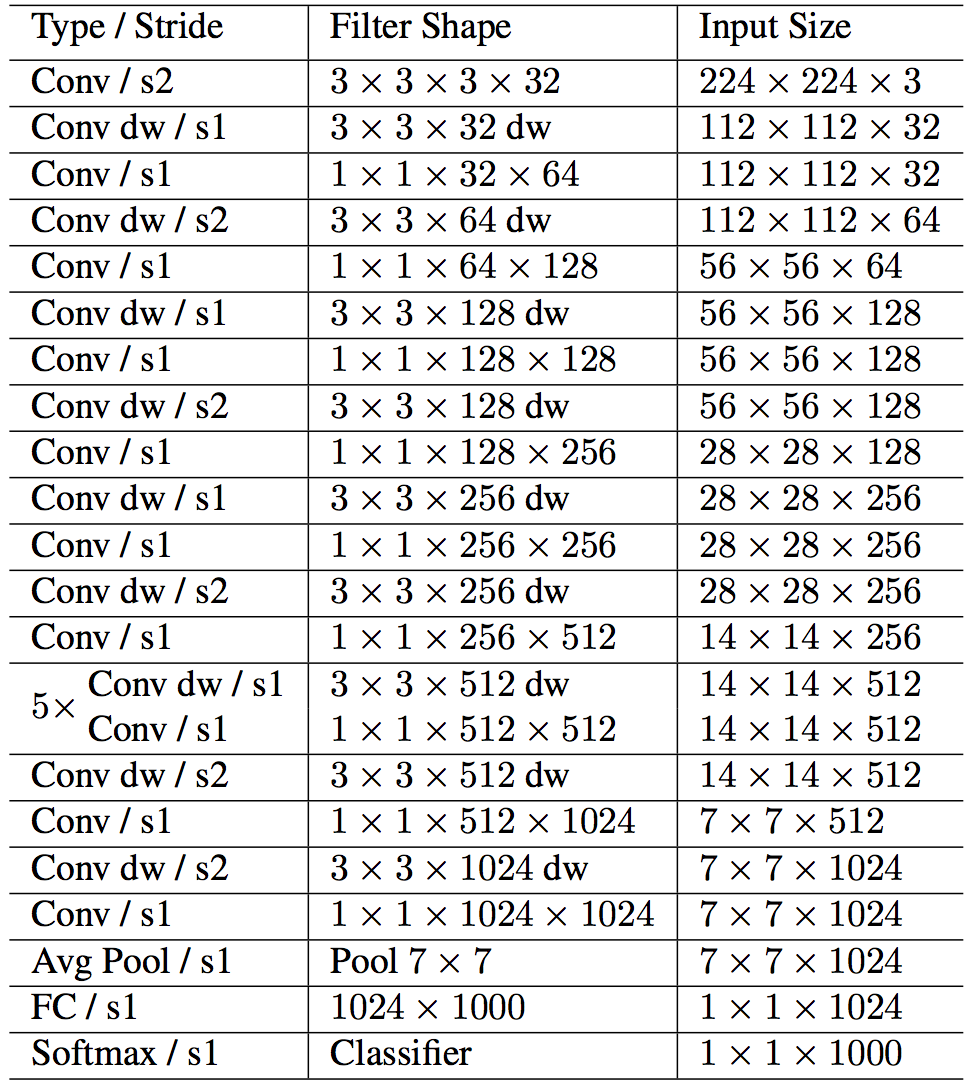
\includegraphics[width=7cm,height=9cm,keepaspectratio]{images/mobileNet_structure.png}
\end{center}
\caption{MobileNet Architecture (Image taken from: \cite{paper:MobileNets}).}
\end{figure}

Each component in the network is followed by a batch-normalization and a rectified linear unit with the sole exception of the final layer which feeds directly into the softmax layer for the classification \cite{paper:MobileNets}. Furthermore, the down sampling is handled with strided convolutions in the depthwise convolutions as well as in the first layer \cite{paper:MobileNets}, while a final average pooling does reduce the overall spatial resolution to 1 before the fully connected layer \cite{paper:MobileNets}. In total the MobileNet counts 28 layers.

\begin{figure}[!htbp]
\begin{center}
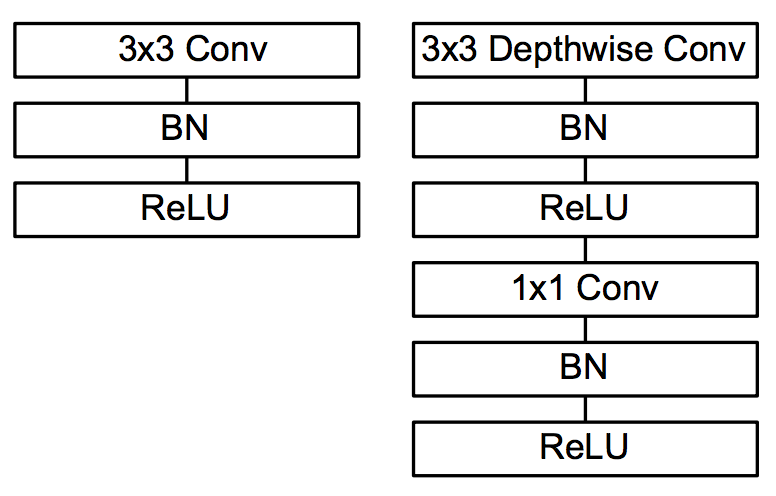
\includegraphics[width=7cm,height=9cm,keepaspectratio]{images/mobileNet_contrast.png}
\end{center}
\caption{Standard convolutional (left), Depthwise Separable convolutions (right) (Image taken from: \cite{paper:MobileNets}).}
\end{figure}

\subsubsection{Depthwise Separable Convolution}

The depthwise separable convolutions is a factorized convolution which factorizes a standard convolution into a depthwise convolution and a 1x1 convolution called pointwise convolution \cite{paper:MobileNets}.

The main difference between a usual convolution and the depthwise one is that the former applies both a filtering and combination procedure to the set of inputs into a new set of outputs in a single step \cite{paper:MobileNets} while the latter splits the procedure into two separate layers. This separation drastically reduces the computation and model size. The figure below shows a standard convolution (a), a depthwise convolution (b) and a 1x1 pointwise convolution (c).

\begin{figure}[!htbp]
\begin{center}
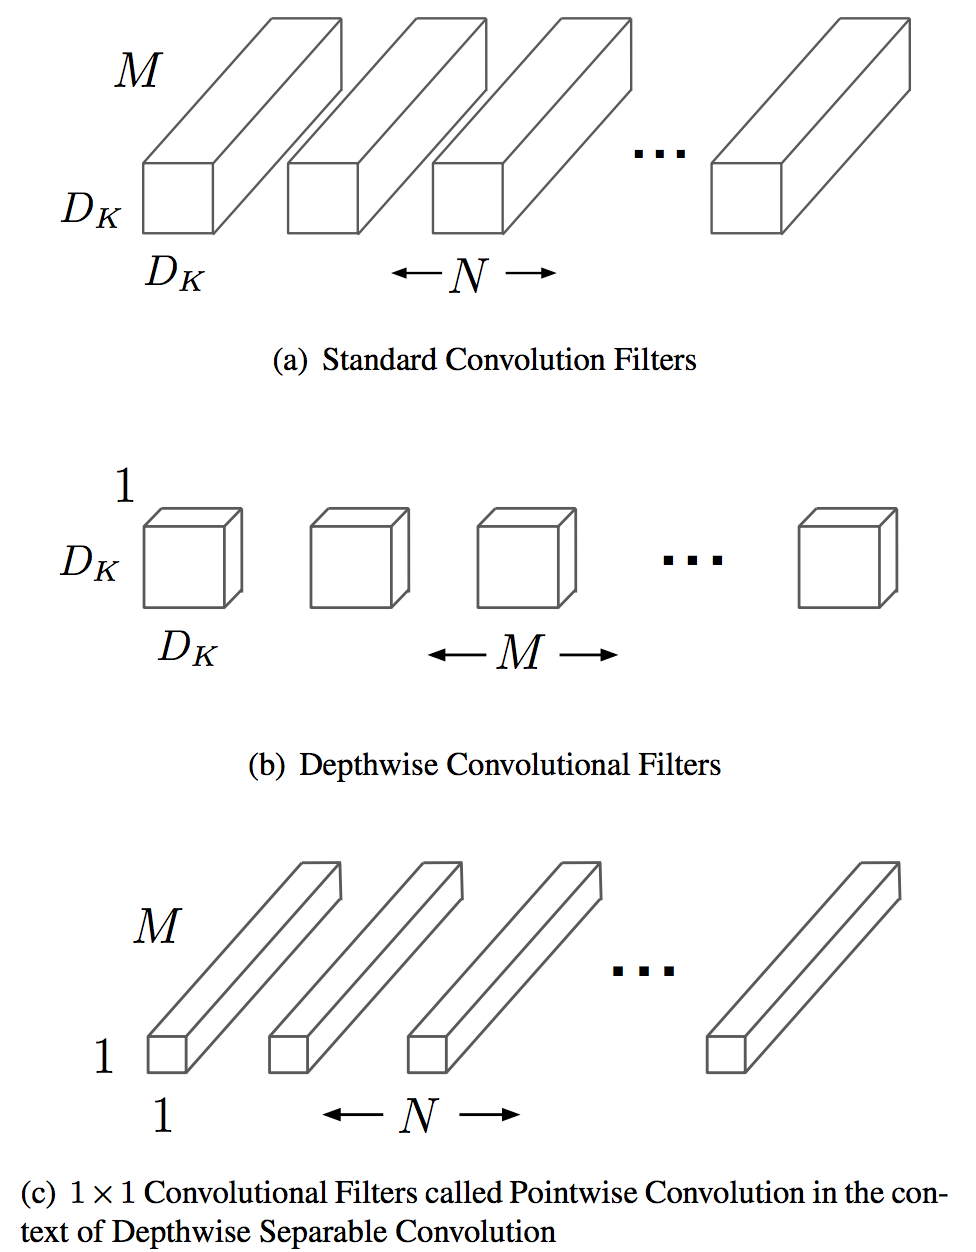
\includegraphics[width=5cm,height=7cm,keepaspectratio]{images/convolutions.png}
\end{center}
\caption{Convolution transformation (Image taken from: \cite{paper:MobileNets}).}
\end{figure}

\subsubsection{Width and Resolution Multipliers}

The basic mobileNet architecture already offers a better efficiency by being smaller and with a lower latency than the usual networks. Nonetheless, many times specif applications require a model which is even smaller and less computationally expensive. The width and resolution hyper-parameters serve exactly this.

The width multiplier defined with the greek letter \textit{alpha} has the role to thin the network layers uniformly \cite{paper:MobileNets}. Usual values for \textit{alpha} are between 0 and 1, with 1 being the model baseline for mobileNet. Moreover, the smaller the parameter gets, the smaller the model will be and hence the less accurate, therefore a trade off has to be found.

The second hyper-parameter to reduce the computational cost of a general neural network is the resolution multiplier defined with the greek letter p \cite{paper:MobileNets}. The parameter is directly applied to the input image and the internal representation of every layer is subsequently reduced by the same multiplier \cite{paper:MobileNets}. Typical values for p are between 0 and 1, with 1 being the mobileNet baseline.

Both parameters reduce the computational cost quadratically.

\begin{figure}[!htbp]
\begin{center}
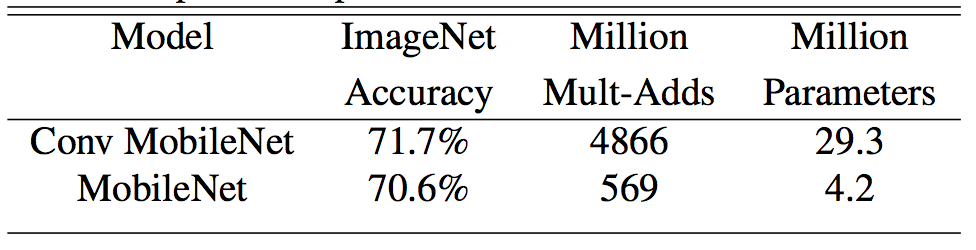
\includegraphics[width=10cm,height=10cm,keepaspectratio]{images/mobileNet_table.png}
\end{center}
\caption{Full vs Depthwise convolutions performance (Image taken from: \cite{paper:MobileNets}).}
\end{figure}

\section{Distance Estimation}

To be able to estimate the position of a person in the final ROS package the only RGB detection is not enough. The distance from the robot to the person is required.

Two main possible approaches have been identified to solve the problem. The first one consists using the RGB-D sensor which comes integrated on TIAGo and which has been presented in Chapter1. The second viable approach consists in using Triangulation, a common vision technique to obtain depth from two or more viewpoints.

\subsection{RGB-D}

The RGB-D camera integrated in TIAGo offers a variety of topics from which valuable sensory data can be retrieved. For the scope of this solution the depth map and the point cloud are the data which we are most interested to, as these respectively offer the distance in millimiters for every RGB pixel and the merge of the RGB and depth data.

Therefore, by leveraging the existing knowledge of where the bounding box depicting the position of humans in the two dimensional RGB array a ROI (Region Of Interest) mapping can be applied, where we try to map the pixels in the RGB where we know a person is present to the corresponding depth pixels.

\subsection{Triangulation}

The problem consists in finding the position of a point in space given its position in two images taken with cameras with know calibration and pose \cite{hartley1997triangulation}. The process requires to find the interesection of the two known rays in space which is trivial when noise is absent, however this is most likely not the case and consequently the rays might never interesect \cite{hartley1997triangulation}. Therefore, it is necessary to find the best possible point \cite{hartley1997triangulation} making of this problem an optimisation one.

The paper presents a solution to the presented problem by assuming a Gaussian noise model for perturbation of the image coordinates, and by formulating it as a least-squares minimisation problem.

\subsubsection{Formulation}

Supposing a point x is present in at least two images and that the two camera matrices P and P' (which define the extrinsic and intrinsic camera information) are known, we identify u and u' to be the projection of such point x in the two images \cite{hartley1997triangulation} and whose intersection is our target.

A commonly suggested method is to choose the midpoint of the common perpendicular to the two rays \cite{hartley1997triangulation}, however such method would not give an optimal result due to the various approximations made \cite{hartley1997triangulation}. Hence a new formulation is made that relies on the concepts of epipolar correspondence and the fundamental matrix \cite{hartley1997triangulation}. The algorithm presented, moreover, is claimed to be moderate in computation requirements due to ist noniterative nature and calculus based approach \cite{hartley1997triangulation}.

\subsubsection{Minimisation Criterion}

The algorithm sets some criteria with regards to the good result of the triangulation process. These are the following:

\begin{enumerate}
  \item The camera matrices and the fundamental matrix are known
  \item The projection points satisfy the fundamental matrix constraint
  \item The image features noise model is a Gaussian
\end{enumerate}

Upon these assumptions the projection points u and u' that are seeked are the ones that minimises the following function \cite{hartley1997triangulation}:

d(u, u')**2 + d(u', u)**2,

where d(*, *) represents the Euclidean distance subject to the epipolar constraint \cite{hartley1997triangulation}:

u'Fu = 0

\section{Leg Detection}

The previously presented literature would surely be enough for a basic human pose estimation, however, this is the case where noise is at its minimum and sensory data are as precise as they can, which is most likely never the case even when using highend hardware. In fact, TIAGo's RGB-D sensor is limited to only an 8m range, hence depth estimation outside the range or even close to the range can be not possible or really noisy.

Therefore the decision to integrate the RGB detection and the RGB-D distance mapping with a leg detector that makes use of 25m range laser-range finder available on TIAGo and supervised learning models to distnguish people's leg in the environment for a more robust pose estimation.

\subsection{Introduction}

Laser range data contain little to no information about people in the environment, as they typically consist of two-dimensional range information \cite{arras2007using}.

\begin{figure}[!htbp]
\begin{center}
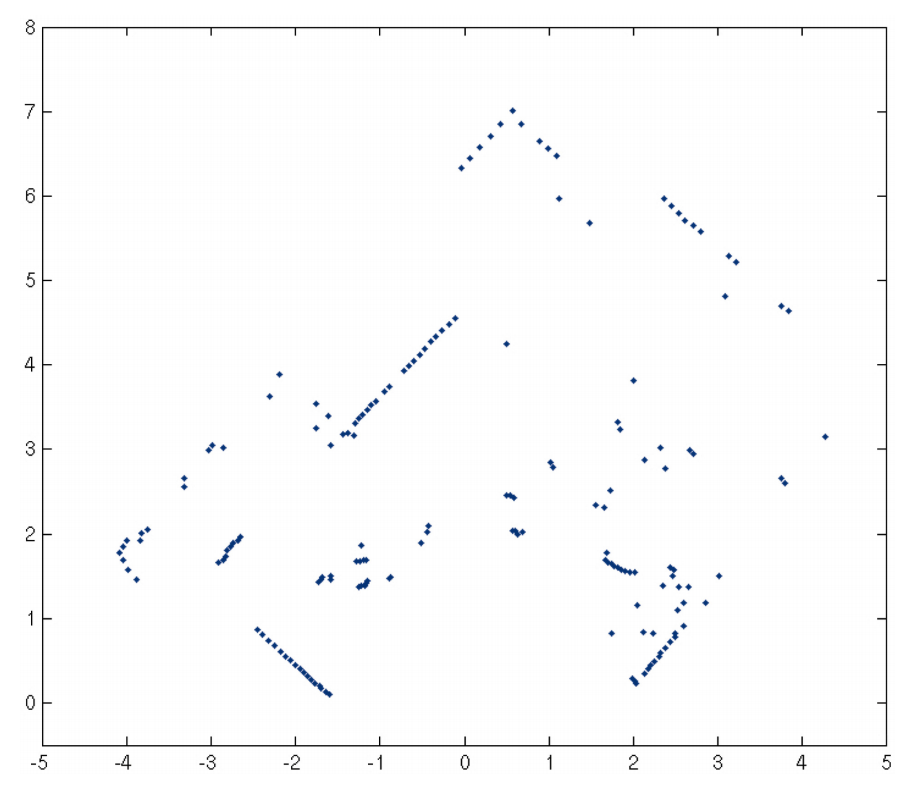
\includegraphics[width=7cm,height=9cm,keepaspectratio]{images/laser-data.png}
\end{center}
\caption{Laser scan data in a typical office (Image taken from: \cite{arras2007using}.}
\end{figure}

The figure above shows the laser scan data returned in a typical office environment. Distinguishing between people's legs and the actual office's objects would be a difficult task for both humans and robots. However, range measurements corresponding to human legs do have certain characteristics, such as size, circularity and convexity \cite{arras2007using}.

The method proposed in the paper aims at defining such set of meaningful scalar features that quantify these properties which can then be detected using an AdaBoost supervised learning approach.

\subsection{Boosting}

Boosting is a general method for creating an accurate classifier by combining a set of weak classifiers \cite{arras2007using}. More precisely, the input to the AdaBoost algorithm used is a set of labeled training data, where each instance is assigned to a weak classifier using a weight distribution over the input \cite{arras2007using}, which ultimately will have a small classification error corrected iteratively by modifying the weight distribution of the examples which were incorrectly classified \cite{arras2007using}. The final strong classifier will be a weighted majority vote of the T best weak classifiers \cite{arras2007using}. In general, we can assume large weights for good weak classifiers and small ones for the poorest \cite{arras2007using}.

\subsection{Features}

The segmentation process is purely done by the robot's hardware in this case. In fact, the returned observations will consist of a set of beams, each one of which is to a tuple containing the angle of the beam relative to the robot and the length of the beam \cite{arras2007using}. Furthermore, the set of beams returned is split on smaller subsets grouped together based on a distance metric such that two adjacent beams are father away than a threshold distance, a new subset is initialised, so that can the segmentations can be readily processed by the subsequent learning step \cite{arras2007using}.

The AdaBoosting algorithm uses 14 different features for the binary classification, where each feature f is defined as a function f:S -> R that takes a segment as an argument and returns a real values \cite{arras2007using}. Below is caption of a laser segment with its feature profile:

\begin{figure}[!htbp]
\begin{center}
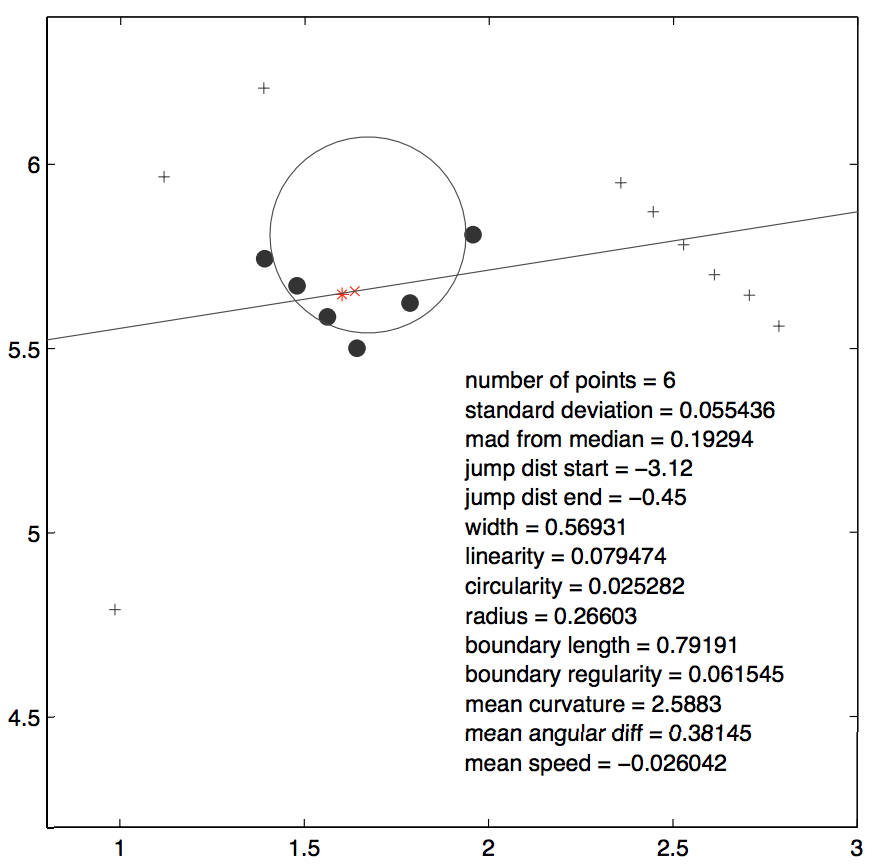
\includegraphics[width=7cm,height=9cm,keepaspectratio]{images/segment_profile.png}
\end{center}
\caption{Segment profile (Image taken from: \cite{arras2007using}.}
\end{figure}

\subsection{Results}

Experimentations with the outlined algorithm were presented in the paper with some excellent results in various cluttered environments like offices and corridors can be, obtaining an encouraging detection rate of over 90\% \cite{arras2007using}.

\begin{figure}[!htbp]
\begin{center}
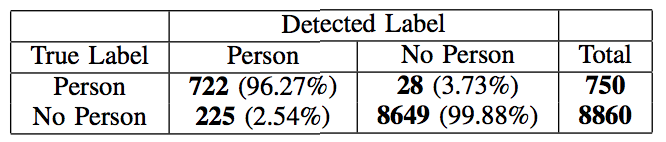
\includegraphics[width=7cm,height=9cm,keepaspectratio]{images/leg_cfm.png}
\end{center}
\caption{Confusion Matrices in office and corridor environments (Image taken from: \cite{arras2007using}.}
\end{figure}




